\documentclass[a4paper,12pt]{article}
\usepackage[utf8]{inputenc}
\usepackage[french]{babel}
\usepackage[T1]{fontenc}
\usepackage[top=2cm,bottom=2cm,left=2cm,right=2cm]{geometry}
\usepackage{graphicx}
\usepackage{wrapfig}
\usepackage{float}
\usepackage{enumitem}
\usepackage{pifont}
\usepackage{fancyhdr}
\usepackage{hyperref}
\usepackage{xcolor}
\usepackage{titling}
\usepackage{amsmath}
\usepackage{algpseudocode}
\usepackage{algorithm}
\usepackage{float}

\definecolor{light-gray}{gray}{0.85}

\newcommand{\subtitle}[1]{
  \posttitle{
    \par\end{center}
    \begin{center}\large#1\end{center}
    \vskip0.5em}
}

\algnewcommand\algorithmicforeach{\textbf{for each}}
\algdef{S}[FOR]{ForEach}[1]{\algorithmicforeach\ #1\ \algorithmicdo}

\title{Rapport de projet}
\subtitle{Sokoban}
\author{Legot Quentin 06.13.45.06.86,\\
Page Arthur 07.68.88.61.20,\\
Besevic Ivan 06.37.72.82.73,\\
Couture Thorkil}

\pagestyle{fancy}
\renewcommand\footrulewidth{1pt}
\fancyfoot[L]{}
\fancyfoot[C]{}
\fancyfoot[R]{Page \thepage}
\begin{document}
\begin{figure}
 \centering
 
\includegraphics[width=0.7\linewidth]{Illustrations/unicaen.png}
\end{figure}

\maketitle

\begin{center}
\href{http://www.unicaen.fr}{\textbf{Université de Caen Normandie}}
\end{center}


\newpage

\tableofcontents

\newpage


\section{Introduction}
\subsection{Explication du projet}

Le but de notre projet était de créer un jeu de type « Sokoban » à la fois fonctionnel et riche. Une fois le jeu de base terminé, nous avons décidé d’ajouter diverses fonctionnalités telles que le jeu contre un ordinateur, la génération aléatoire de niveaux et le comptage des points. Nous avons par ailleurs mis en place des niveaux de difficulté pour rendre le jeu accessible à tous et ainsi éviter d’avoir un contenu trop monotone. Nous avons partagé le travail à quatre pour que chaque membre puisse ajouter sa touche personnelle au jeu. Nous allons donc ici vous parler du jeu en lui-même (ses principes de base et ses mécaniques), des étapes de la conception et des différentes fonctionnalités que nous avons ajouté au jeu de base.

\subsection{Le Sokoban, qu’est-ce que c’est ?}

Créé au Japon en 1982, le Sokoban est un jeu vidéo  de type puzzle à un joueur dans lequel on incarne un ouvrier devant ranger des caisses dans un entrepôt. Le joueur peut se déplacer dans toutes les directions et peut seulement pousser une caisse à la fois. Les déplacements en diagonale ne sont pas possibles et le joueur ne peut pas tirer de caisses. Dans l’entrepôt, outre les caisses et les murs, se trouvent aussi des points. Pour gagner et finir le niveau, il faut que tous les points soient recouverts par des caisses. Suivant la spécificité du niveau le joueur peut se retrouver bloqué en poussant une caisse dans un coin. Le but du jeu est donc de finir le niveau en effectuant le moins de mouvements possibles.
\begin{figure}[H]
    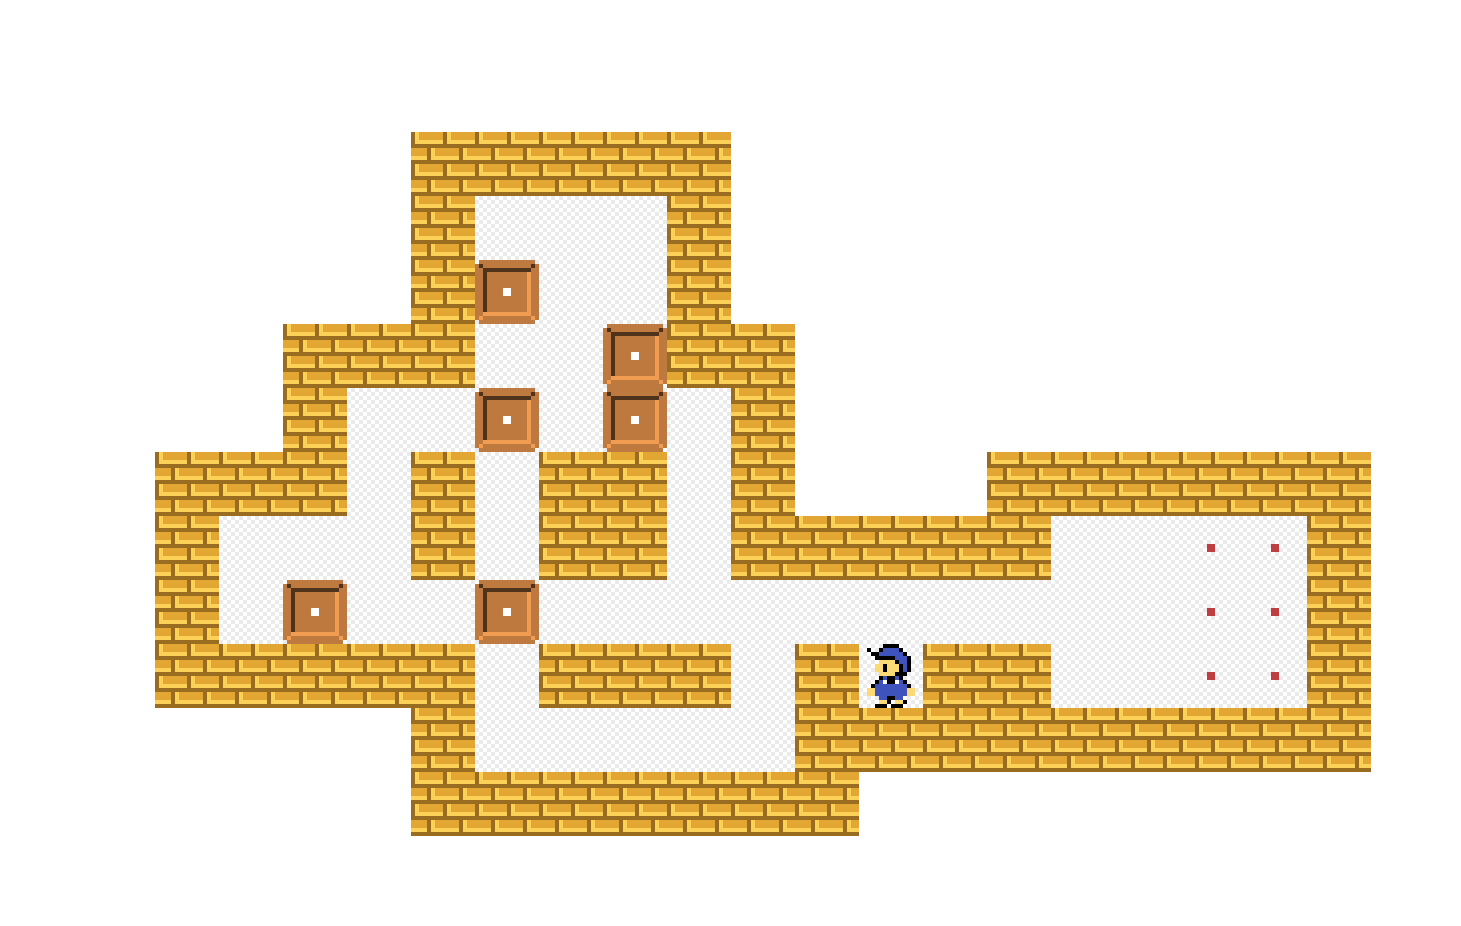
\includegraphics{./Illustrations/Original.png}
    \caption{Premier niveau du jeu original de 1982}
\end{figure}
\newpage
\section{Manuel du jeu}

\subsection{Préambule}

Notre jeu a été développé pour les versions de Python supérieures à la 3.6, aucun test n'a été fait sur les précédentes versions.\\
Le jeu fonctionne sur  Linux avec xorg et Windows 10, aucun test n'a été effectué sur Mac OS X (il peut y avoir des problèmes de dispositions clavier, appuyez sur W au lieu de Z par exemple).\\

\subsection{Lancement du jeu}

Tout d'abord, pour lancer le jeu, sachez qu'il vous faut avoir installé Python ainsi que la bibliothèque Pygame.
Une fois ceci fait, voici les étapes à suivre pour lancer le jeu:\\
\begin{itemize}
    \item Placez vous dans le répertoire racine du jeu, où se trouve le fichier \textit{main.py}.
    \item Ouvrez un terminal et tapez "\textit{python3 main.py}".
    \item  Le jeu se lancera.
\end{itemize} 
Le jeu étant lancé, une fenêtre s'ouvrira, vous menant directement au menu principal du jeu.\\
\begin{figure}[H]
\begin{center}
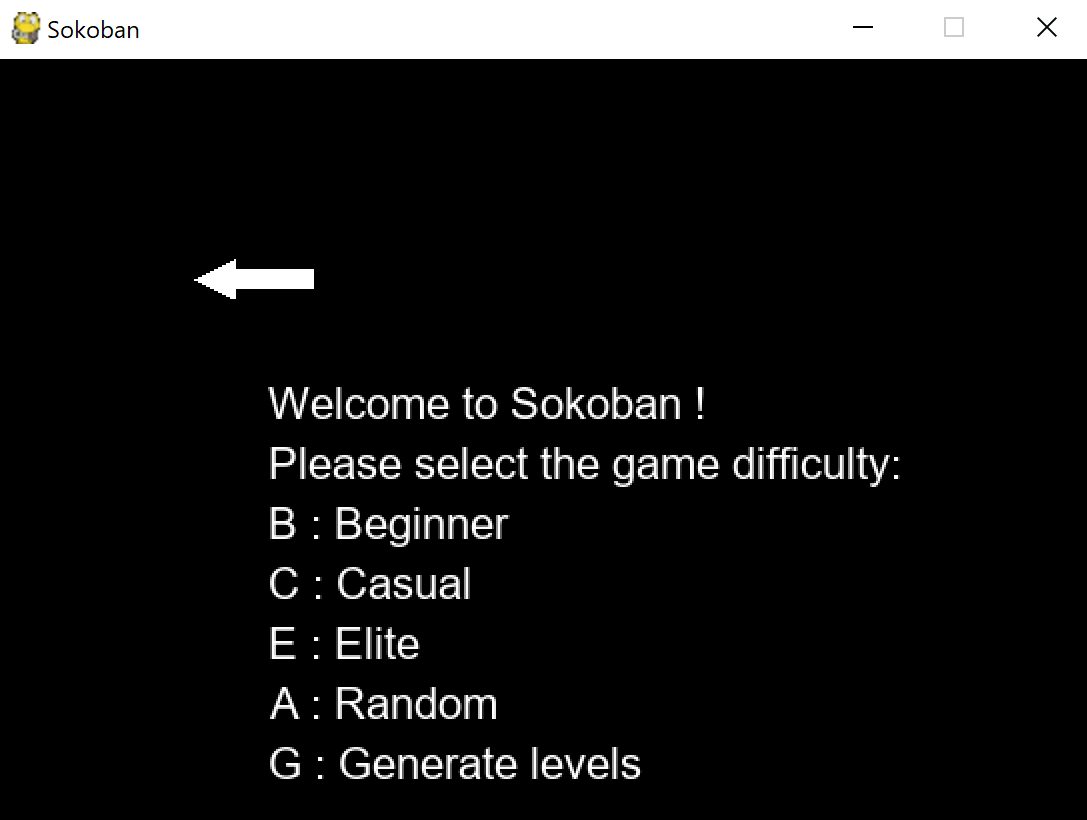
\includegraphics{./Illustrations/menu.png}
\caption{Menu principal du jeu.}
\end{center}
\end{figure}

\subsection{Navigation dans les menus}

La navigation dans les menus se fait à la souris ou au clavier. Si vous utilisez la souris, cliquez simplement sur les lignes voulues; pour le clavier, il faut appuyer sur les touches indiquées à gauche des lignes. Pour les nombres, utilisez le pavé numérique ou faites \textit{shift} + \textit{NUM} si votre PC n'en est pas équipé.\\
Appuyez sur \textit{ECHAP} ou sur la flèche qui va vers la gauche pour revenir en arrière ou quitter le jeu si vous êtes sur le premier écran. Vous pouvez appuyez sur la croix de la fenêtre pour quitter le jeu à tout moment.

\subsection{Choix du niveau}

Vous voulez jouez tout de suite ? Pas de problème, suivez simplement les étapes suivantes:
\begin{enumerate}
    \item Choisissez le mode de jeu le plus adapaté ( \textit{Beginner , Casual , Elite} ou \textit{Random}).
    \item Pour les trois premier choix, plusieurs niveaux s'offrent à vous, classés du plus simple au plus compliqué.
    \item Pour le quatrième choix (\textit{Random}), une grille sera crée selon vos préférences, vous n'avez qu'à entrer le nombres de caisses avec lesquelles vous souhaitez jouer (de 1 à 9).
    \item Dernière étape enfin, vous devrez choisir si vous jouerez contre un ami (\textit{Versus Player}), ou contre l'ordinateur (\textit{Versus Computer}).
\end{enumerate}
\begin{figure}[H]
\begin{center}
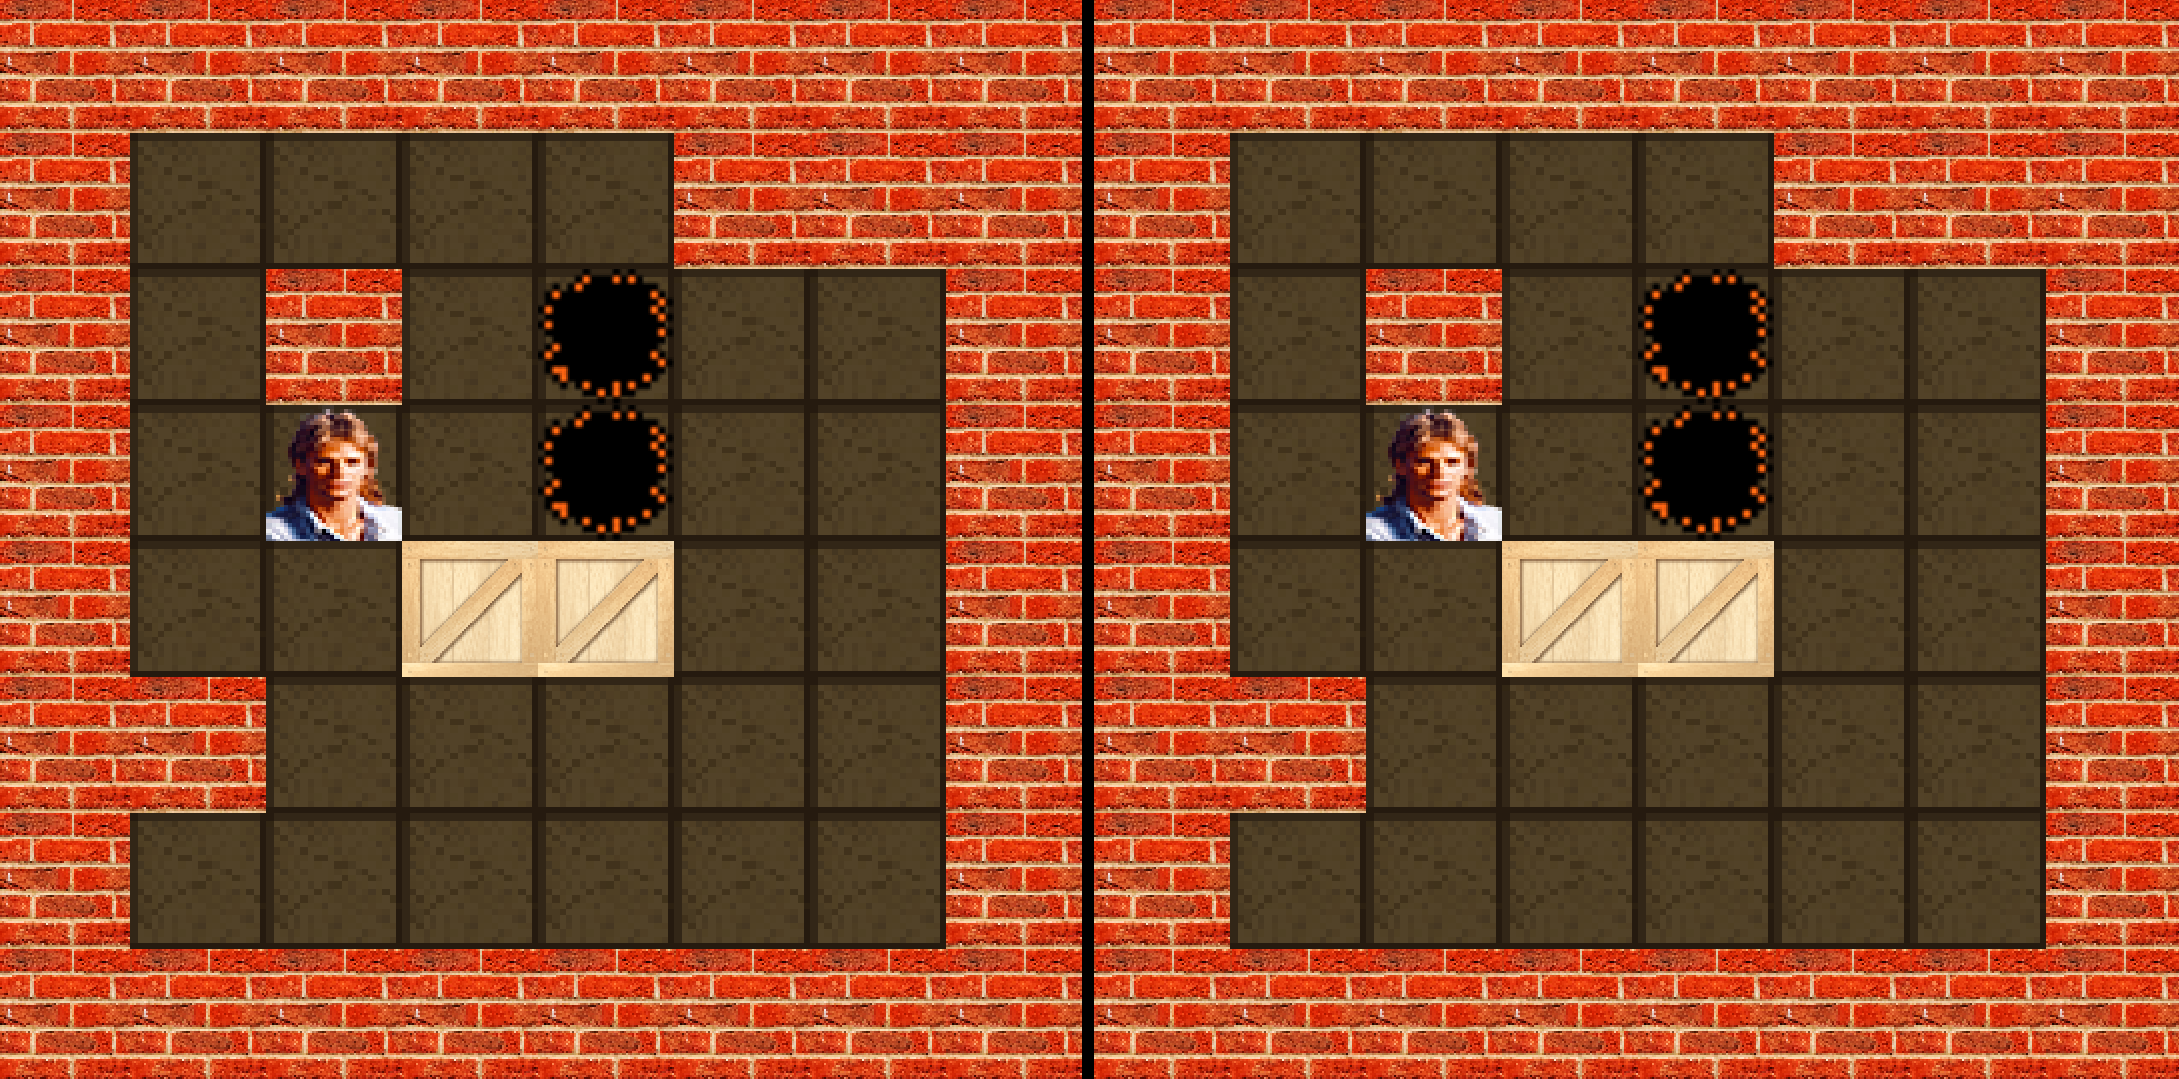
\includegraphics[scale=0.4]{./Illustrations/splitscreen.png}
\caption{Début de partie en mode deux joueurs. Difficulté: \textit{Beginner}. Niveau: \it1}
\end{center}
\end{figure}
\subsection{Comment jouer ?}
Si vous avez suivi les étapes précédentes, vous devriez voir apparaître la grille de jeu. Nous arrivons donc enfin à la partie la plus intéressante, comment jouer.
\begin{itemize}
\item Si vous jouer contre un ami, sachez que le joueur de gauche déplacera son personnage grâce au touches "\textit{z,q,s,d}", respectivement "\textit{haut, gauche,bas,droite}", et que le joueur de droite se servira des flèches du clavier. Le but, en mode deux joueurs est donc de placer toutes les caisses sur les trous en essayant de se déplacer au minimum. Ainsi le joueur ayant effectué le moins de coups pour placer ses caisses gagne la partie. Une fois la partie terminée, le nom du vainqueur est affiché et vous retournez automatiquement au menu principal.
\item Si vous jouez contre l'ordinateur, vous devrez utiliser les touches "\textit{z,q,s,d}" pour vous déplacer. L'ordinateur joue en même temps que vous (il se déplace quand vous vous déplacez) mais si jamais vous avez fini avant lui de placer toutes vos caisses, alors il finira sa partie automatiquement après vous.\\
\item Sachez que si vous en avez assez de perdre ou tout simplement que le jeu vous ennuie, vous pouvez quitter à tout moment la partie grâce à la touche "\textit{echap}" de votre clavier.
\end{itemize}
\subsection{"\textit{Generate levels}"}
Vous avez sûrement dû vous rendre compte qu'une rubrique "\textit{Generate levels}" est présente dans le menu du jeu. Vous pouvez y accéder en cliquant dessus ou en pressant la touche "\textit{g}" de votre clavier.\\
Cette option permet de renouveler les niveaux du jeu entièrement. La méthode est la suivante:
\begin{itemize}
    \item Tous les niveaux du jeu seront supprimés.
    \item Des niveaux seront créés grâce au générateur de niveaux (cf. Générateur \ref{gen}).
    \item Ses niveaux seront ensuite testés par le solveur pour voir si il peut les résoudre (cf. Solveur \ref{section::solveur}).
    \item Si les niveaux sont résolvables par le solveur, alors ils prennent la place des anciens niveaux du jeu.
\end{itemize}
Tous les niveaux du jeux étant recrées, l'opération nécessite un certain temps. Nous vous conseillons donc de n'utiliser cette fonctions qu'en dernier lieu, lorsque vous vous serez lassé des niveaux actuels du jeux.

\newpage

\section{Conception du jeu}
\subsection{Organisation du projet}

Voici la manière dont nous nous sommes réparties les tâches du projet. L'un de nos membres (COUTURE Torkil) nous ayant quitté en cours de projet, nous n'avons pas pu mentionner son nom dans ce tableau.\\
\begin{center}
\begin{tabular}{|c|c|c|c|c|}\hline
Fonctionnalités principales&Affichage&Solveur&Générateur\\ \hline\hline
Ivan&      Ivan&      Quentin&      Arthur   \\\hline
\end{tabular}
\end{center}

\subsection{Fonctionnalités}

\subsubsection{Les états du programme}

Pour que l’enchaînement des différentes mises en page du sokoban soient cohérentes, j'ai décidé de créer un fichier logic/state.py qui posséderait toutes les informations liées à l'état du programme avec des fonctions permettant de manipuler ces états.\\

Ce programme possède quatre situations possibles :

\begin{figure}[H]
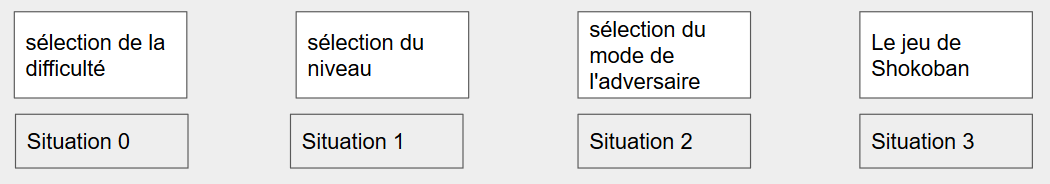
\includegraphics[width=\linewidth]{./Illustrations/state_1.png}
\caption{Principales situations.}
\end{figure}

Ces situations se suivent de manière logique :\\

\begin{figure}[H]
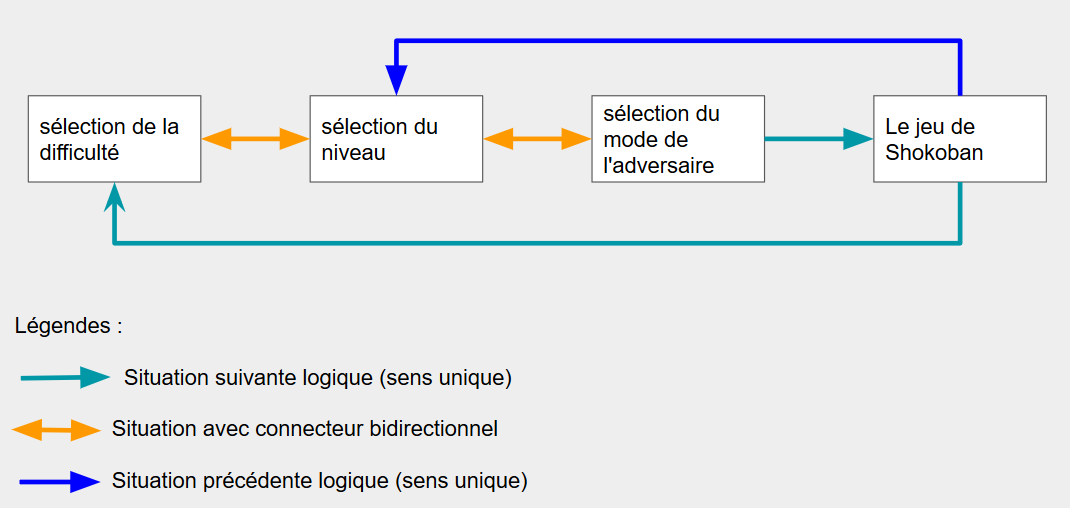
\includegraphics[width=\linewidth]{./Illustrations/state_2.png}
\caption{Suivi des situations.}
\end{figure}

C'est la classe de state.py qui analyse les événements Pygame afin de prendre les bonnes décisions pour modifier l'état du jeu.\\
Ces événements Pygame vont donc modifier des variables python représentant l'état du jeu en fonction de la situation.\\

Celles-ci sont représentées par le schéma suivant :

\begin{figure}[H]
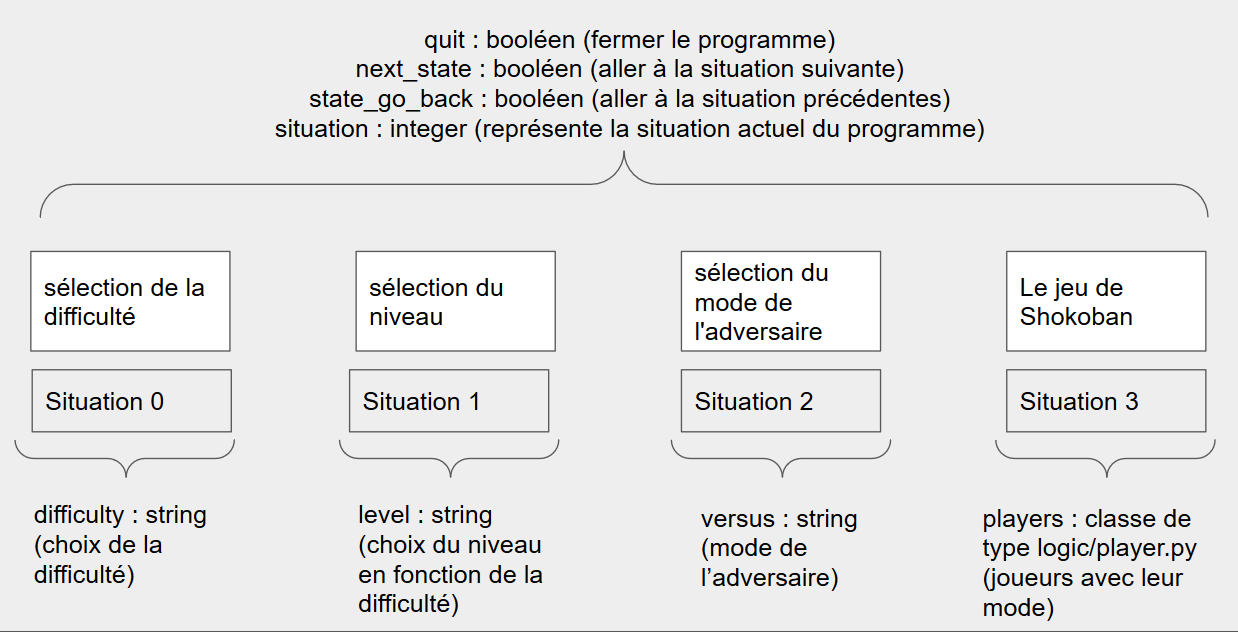
\includegraphics[width=\linewidth, height=3in]{./Illustrations/state_3.png}
\caption{Variables python modifiées selon la situation.}
\end{figure}

Chaque situation écoute des événements Pygame qui leur sont propres.\\
Dans notre jeu, nous écoutons uniquement les touches du clavier et de la souris (en prenant en compte la position pour la souris).

Les événements écoutés sont représentés par le schéma suivant :

\begin{figure}[H]
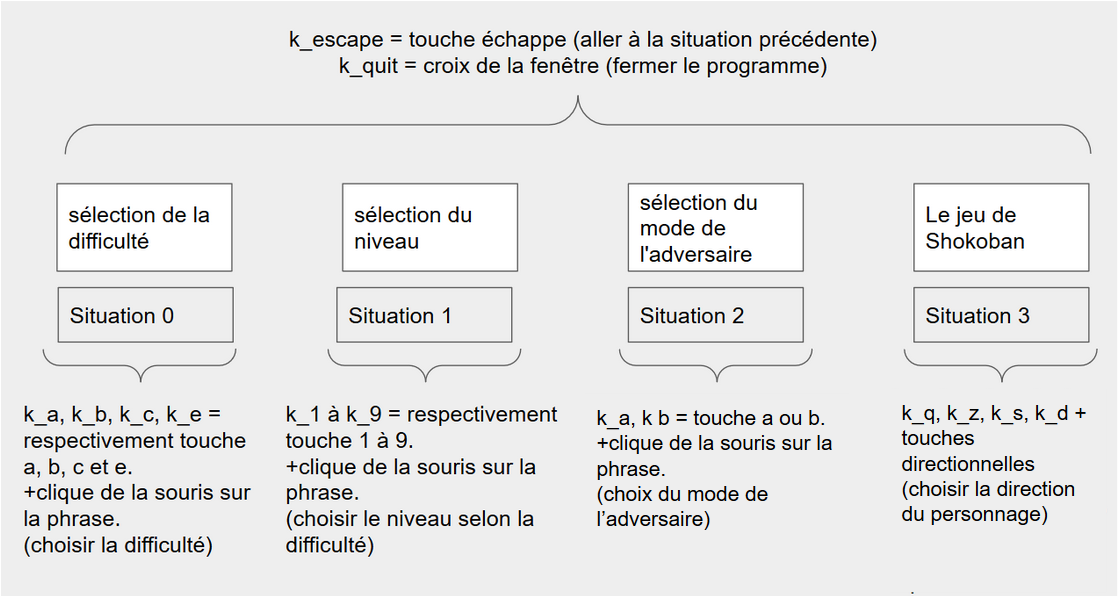
\includegraphics[width=\linewidth]{./Illustrations/state_4.png}
\caption{Les événements écoutés selon la situation.}
\end{figure}

\newpage

\subsubsection{Le rendu du jeu}

Une fois que l'utilisateur arrive dans la situation de jeu,
la classe de logic/state.py va demander la génération des classes players de logic/player.py.\\

Cette classe player va à son tour demander la création d'une grille spécifique aux joueurs.\\
Dans le programme on a donc une grille indépendante par joueur.\\

Tout d'abord une grille de lettres va être créée à partir d'une génération automatique (cf. La partie d'Arthur Page \ref{gen}) ou d'un fichier .sok.\\

Dans ma partie, je vais vous parler de la création de la grille à partir des fichiers .sok.\\

Voici le contenu d'un fichier .sok :

\begin{figure}[H]
\begin{center}
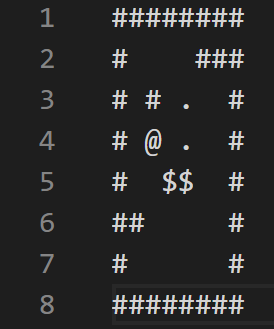
\includegraphics[width=2.5in, height=2.5in]{./Illustrations/map_1.png}
\end{center}
\caption{Contenu d'un fichier .sok.}
\end{figure}

Celui-ci va être converti en grille de lettres :

\begin{figure}[H]
\begin{center}
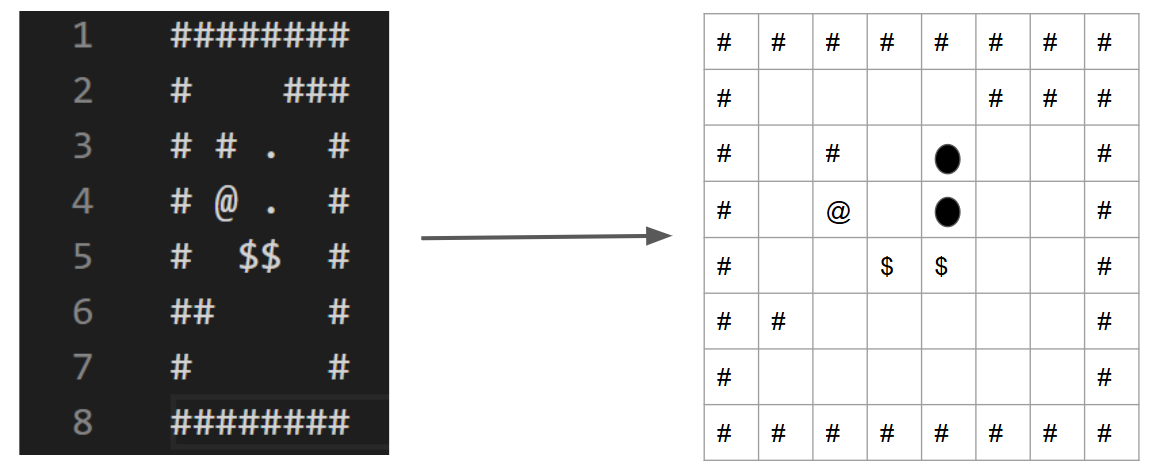
\includegraphics[width=5in]{./Illustrations/map_2.png}
\end{center}
\caption{Conversion fichier .sok en grille python.}
\end{figure}

Ensuite chaque lettre de la grille va être convertie en un sprite Pygame qui lui est associé.\\

\begin{figure}[H]
\begin{center}
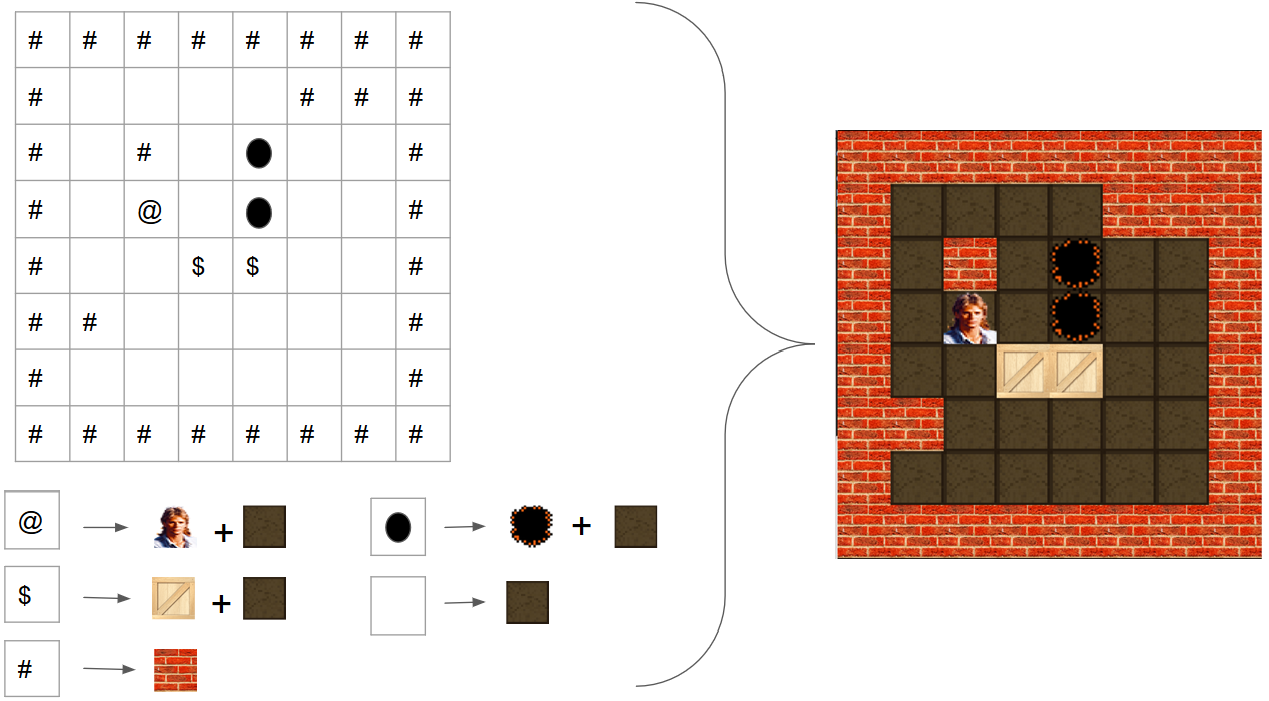
\includegraphics[width=7in, height=3.7in]{./Illustrations/map_3.png}
\end{center}
\caption{Conversion des lettres de la grille en sprites.}
\end{figure}

On a deux types de sprite Pygame dans le programme :
\begin{itemize}
\item Les sprites superposables [joueur(@), boites(\$), trous(.), air( )]
\item Les sprites non superposables [mur(\#)]
\end{itemize}

\vspace{5mm}

Pour positionner les sprites sur la fenêtre Pygame, nous avons dû effectuer des mesures sur la/les grilles.

\begin{figure}[H]
\begin{center}
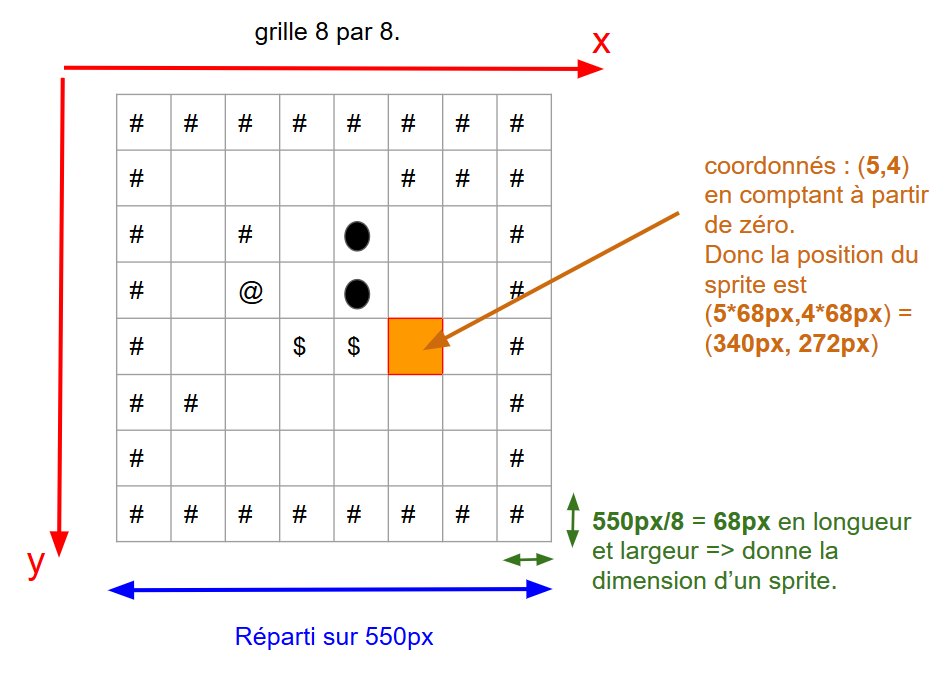
\includegraphics[width=6in, height=3.6in]{./Illustrations/map_4.png}
\end{center}
\caption{Mesures effectuées pour chaques sprites de la grille.}
\end{figure}

Une fois que tout est en place le programme situé dans interface/screen.py peut afficher le rendu des sprites à partir de leur positions calculés.

\subsubsection{Mouvement du personnage dans la grille}

Le personnage se déplace uniquement de une case, en verticalement ou horizontalement.
Les mouvements du personnage sont restreints par des règles.

Voici un contexte, représenté par le schéma suivant :

\begin{figure}[H]
\begin{center}
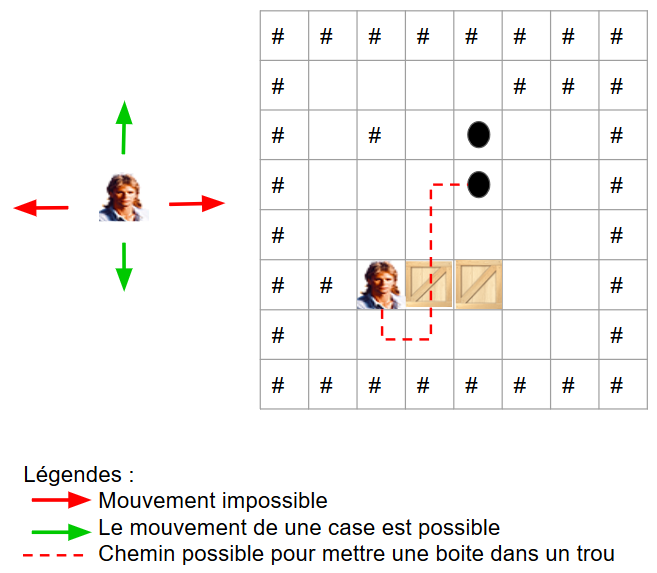
\includegraphics[width=6in, height=3.6in]{./Illustrations/mouv_1.png}
\end{center}
\caption{Les mouvements possibles du personnage dans la grille.}
\end{figure}

La logique liée au mouvement respecte le pseudo-code suivant : 

\begin{figure}[H]
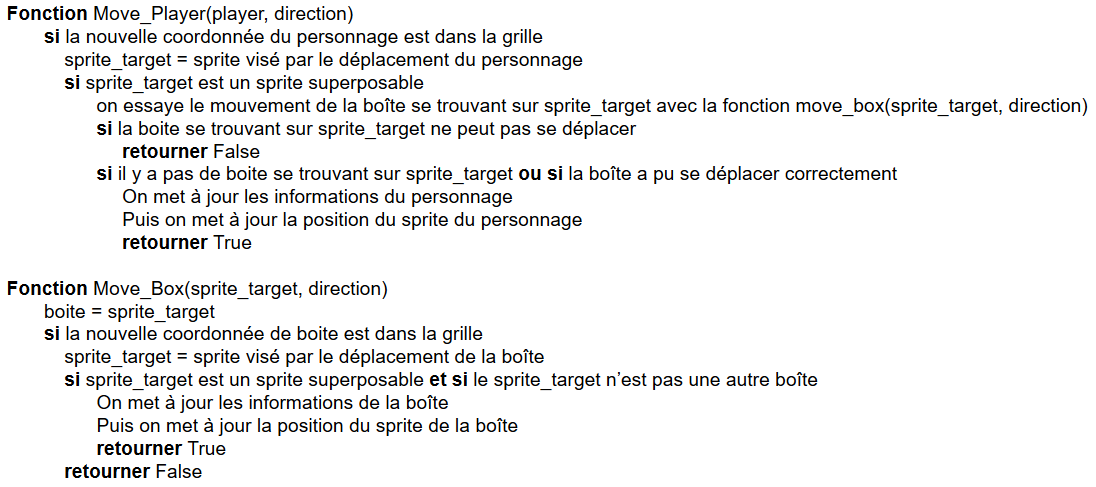
\includegraphics[width=\linewidth]{./Illustrations/mouv_2.png}
\caption{Pseudo-code du déplacement du personnage dans la grille.}
\end{figure}

\subsubsection{Solveur}
\label{section::solveur}
Le solveur se découpe en 2 parties: l'algorithme A* qui permet de trouver le chemin le plus court en partant d'un point A pour aller à un point B et la classe solver en elle-même qui va essayer de résoudre le niveau.\\
Dans un premier temps, le solveur essaie de chercher la caisse qui se trouve la plus proche du joueur et va essayer de trouver un chemin vers le point de validation(traits gris) puis on calcule le chemin de la caisse vers le point grâce à l’algorithme A* pour vérifier que la caisse peut effectivement se placer dessus(traits verts).\\
S'il y arrive on va réutiliser l'algorithme A* pour déterminer le chemin que doit parcourir le personnage pour aller jusqu'à la caisse (traits jaunes). On calcule ensuite le chemin que doit parcourir le personnage pour pouvoir pousser la caisse jusqu'au point (traits rouges), et on ajoute l'emplacement de la caisse en mémoire pour que l'algorithme A* soit informé qu'il ne peut plus traverser cet emplacement.

\begin{figure}[H]
\begin{center}
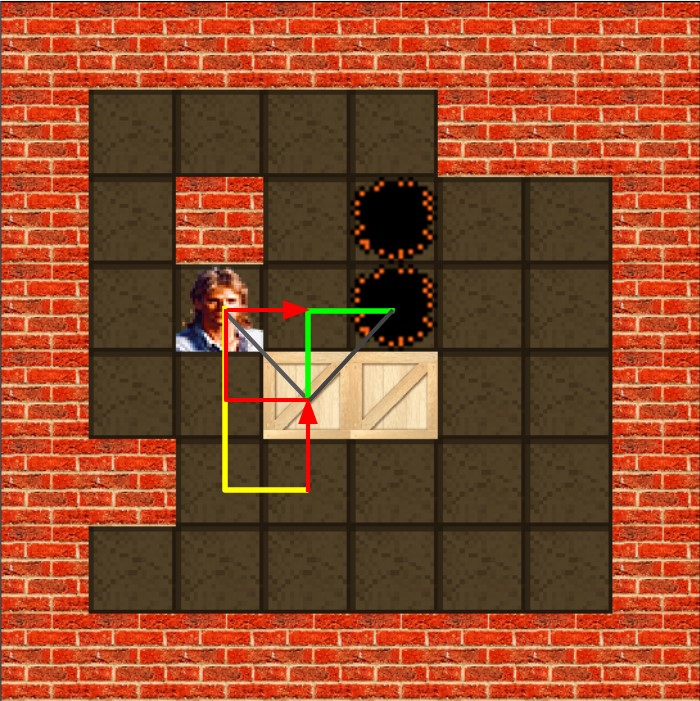
\includegraphics[width=0.6\linewidth]{./Illustrations/solver1.jpg}
\caption{Tout les chemins / calculs effectués par le solveur pour placer la première caisse}
\end{center}
\end{figure}

En effet, l’algorithme ne change pas la disposition du terrain au fur et à mesure de son exécution afin que ce changement se fasse en temps réel, quand le joueur joue et se déplace. Nous stockons donc le terrain de base ainsi que 2 listes de Tuples qui servent à dire à l’algorithme A* qu'il peut traverser une caisse (étant donné que nous ne changeons pas la disposition du terrain s'il bouge la caisse il peut à nouveau se poser sur cet emplacement) et l'autre qui sert au contraire à dire à l'algorithme A* qu'il ne peut plus traverser tel ou tel emplacement.\\

Dès que la caisse se trouve à l’emplacement voulu on cherche à nouveau la caisse la plus proche et le point de validation le plus proche de cette caisse (traits gris), on calcule le chemin de la caisse(traits verts). On approche ensuite le joueur de la caisse(trait jaune), on détermine le chemin à suivre grâce à l'algorithme(traits rouges) et on répète ses étapes jusqu'à ce qu'il ne reste plus un seul point de validation valide.

\begin{figure}[H]
\begin{center}
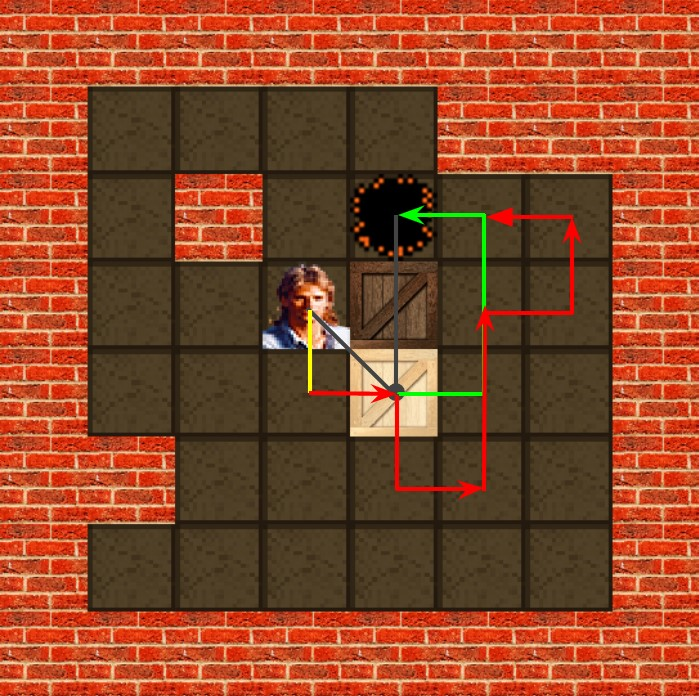
\includegraphics[width=0.6\linewidth]{./Illustrations/solver2.jpg}
\caption{Calculs effectués pour déplacer la seconde caisse}
\end{center}
\end{figure}

\begin{figure}[H]
\begin{algorithmic}
\Function{solveur}{grid, From:Node, Goal:Node}\\
\State $closedList = []$
\State $openList = []$ \Comment{File prioritaire}
\State $came\_from = \{\}$
\State $openList.add(From)$
\While{openList is not empty}
	\State $current\_node = openList.popTHeSmallestItem()$
	\If {$current\_node['x'] == NoeudArrive['x'] $ }
		\State \Return constructPath()
	\EndIf
	\ForEach{$current\_node\: neighbor \in grid$}
		\If{$not(neighbor\in closedList\:\|\:(neighbor \in openList\:\&\:neighbor.cost \leq getNeighborFromOpenList().cost))$}
			\State $neighbor.cost = current_node[''cost''] + 1$
			\State $neighbor.heuristic = neighbor.cost * (|neighbor.x - Goal.x| + |neighbor.y - Goal.y|)$
			\State $current\_node.append(neighbor)$
		\EndIf
	\EndFor
	\State  $closedList.append(current_node)$
\EndWhile
\State Raise Exception
\EndFunction
\end{algorithmic}
\caption{Algorithme A*}
\end{figure}
% https://en.wikibooks.org/wiki/LaTeX/Algorithms#Typesetting_using_the_algorithmicx_package

\subsubsection{Générateur}
\label{gen}
Pour éviter de rendre le jeu lassant et augmenter sa durée de vie, il nous est venu comme idée d'implémenter un générateur de niveaux. Il sera expliqué dans cette section le fonctionnement du générateur ainsi que ses particularités. \\
Le générateur peut se configurer de plusieurs manières. On peut ainsi choisir un nombre de caisses maximum et un nombre de caisses minimum, ainsi que la taille de la grille et la difficulté. Nous allons donc voir étape par étape en quoi chacun de ses paramètres intervient dans la génération d'une grille.\\
On notera que pour des raisons de simplicité, toutes les grilles générées sont des grilles carrées.\\
Voici comment le générateur construit une nouvelle grille:
\begin{enumerate}
\item Création de la grille de base.
\item Remplissage de la grille.
\item Vérifications.
\end{enumerate}
\paragraph{Création de la grille de base}
\paragraph{}
Le générateur créé tout d'abord une grille carrée de la taille demandée. Il fait en sorte que cette grille soit seulement constituée de murs en faisant le tour; le reste de la grille étant vide.\\
Il initialise aussi trois dictionnaires dans lesquels seront stockées les positions du joueurs, des caisses et des trous.

\paragraph{Remplissage}
\paragraph{}
Une fois cette grille créée, le générateur doit la remplir. Il affecte à des variables le nombre de caisses et de trous qu'il doit placer. Une variable contenant le nombre de murs est aussi créée, elle contient un nombre correspondant au à la moitié de la taille de la grille multiplié par la difficulté. Plus un niveau est difficile, plus il contient donc de murs.\\
Le générateur remplit ensuite la grille en excluant le deux premières lignes (\textbf{resp.} colonnes) de chaque colonnes (\textbf{resp.} colonnes). L'exclusion de ses cases permet d'éviter que les caisses ne se retrouvent accolées aux murs extérieurs de la grille (ce qui rendrait la génération des trous plus contraignante).\\
Le générateur utilise la fonction "\textit{randrange}" du module "\textit{random}" de Python pour choisir au hasard où il doit placer une caisse un mur ou un trou. Si la case choisie contient déjà un objet, le générateur en choisit une autre, et continue de choisir au hasard des cases jusqu'à ce que tous les objets soient placés.\\
Le générateur place dans cet ordre, le joueur, puis les murs, suivis des caisses et en dernier les trous.\\
Une fois placé, un objet voit sa position ajoutée dans son dictionnaire correspondant pour faciliter l'étape de vérification.
On obtient donc un algorithme de ce genre pour un objet :\\
\begin{algorithmic}
\While{$nombre d' objet \neq 0$}
    \State $x\gets randrange(2,tailledelagrille -3)$
    \State $y\gets randrange(2,tailledelagrille -3)$
    \If {$grille[x][y] =  empty$}
        \State $grille[x][y] \gets objet$
        \State $nombred'objet \gets nombred'objet - 1 $
        \State $DicObjet[objet] \gets [x,y]$
    \EndIf
\EndWhile
\end{algorithmic}
\paragraph{Vérification}

Une fois tous les objets placés sur le grille, le générateur procède à plusieurs vérifications pour voir si la grille est conforme à certains critères. Ainsi si une case vide est entourée de murs, elle sera transformée en mur.\\
D'autres test sont rédhibitoires. Si ils ne sont pas valides, le générateur recommence à générer une grille depuis le début (retour à la création de la grille de base).\\
On distingue trois de ces tests:
\begin{itemize}
    \item Si une caisse est entourée par plus de deux murs.
    \item Si il n'y a pas autant de caisses que de trous.
    \item Si il n'y a pas exactement un joueur.
    \item Si il y a moins de boîtes que demandé en appel de la classe.
\end{itemize}
Pour rendre l'exécution des vérifications plus rapide, les dictionnaires contenant les positions des objets de la grille sont utilisés, pour éviter de devoir parcourir la grille afin de les trouver.\\
Si tous ces tests renvoient la valeur "\textit{True}", alors la grille est considérée comme valide et la classe \textit{Generate} la retourne.

\begin{figure}[H]
\center
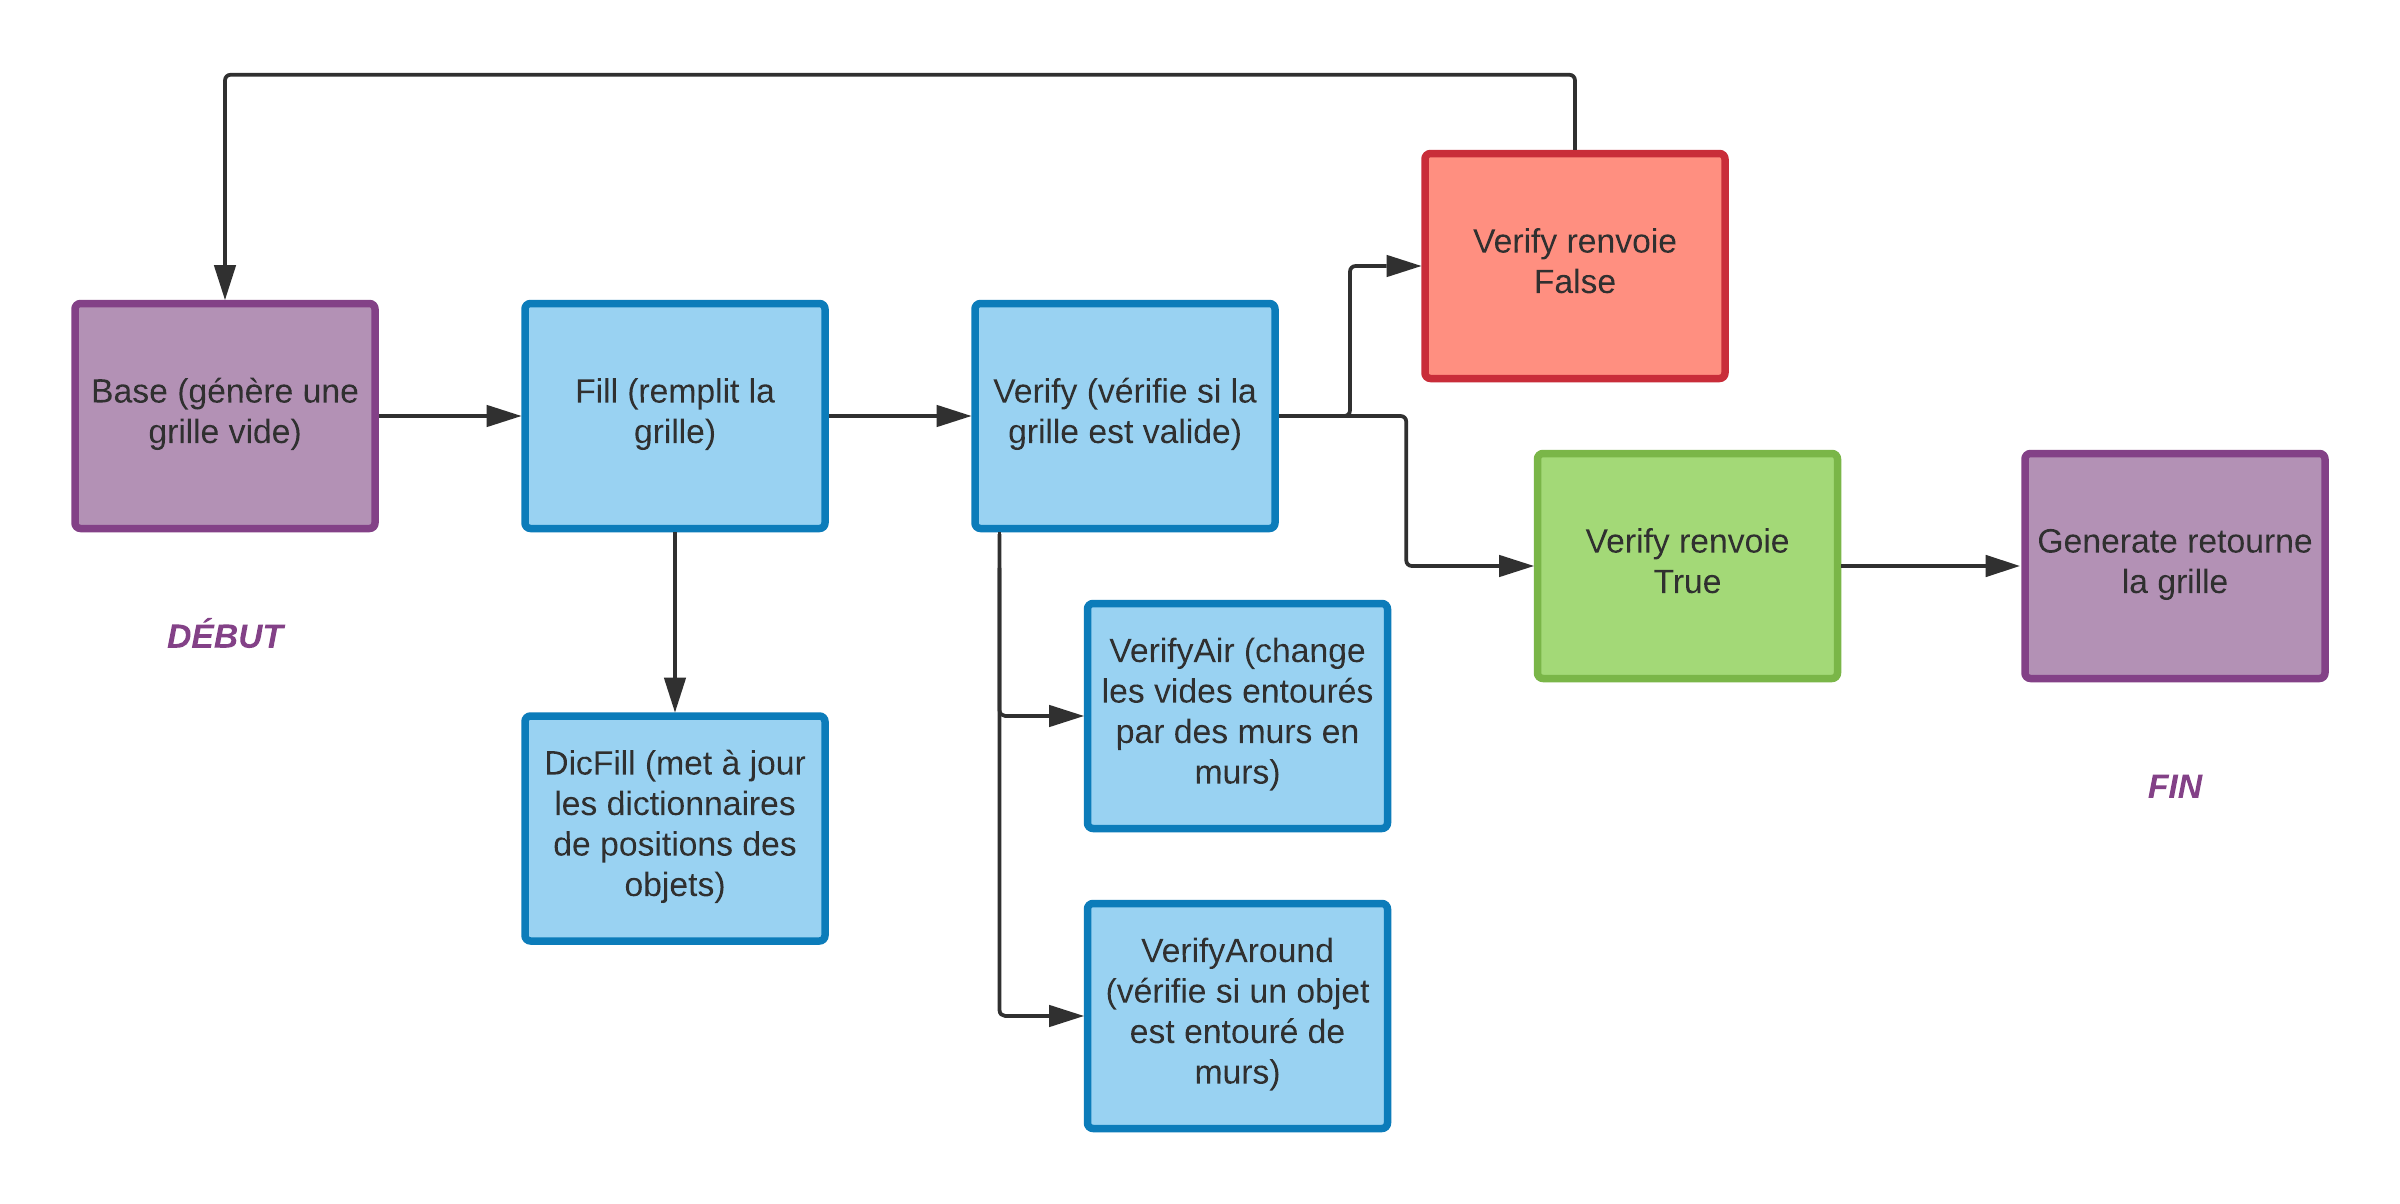
\includegraphics[scale = 0.90]{./Illustrations/generate.png}
\caption{Fonctionnement de la classe Generate.}
\end{figure}

\newpage

\section{Éléments techniques}
\subsection{Structure de données}

Explication de l'organisation des dossiers :
\begin{itemize}
  \item{Config}
    \begin{itemize}
      \item{Contient les constantes utile au fonctionnement du jeu.}
      \item{Le chemin absolu du répertoire du dossier parent afin de pouvoir récupérer facilement les fichiers .sok qui contiennent les schémas des labyrinthes.}
      \item{Le titre et les dimensions de la fenêtre.}
      \item{L'identifiant de notre Event pygame personnalisé.}
    \end{itemize}
  \item{Images}
    \begin{itemize}
      \item{Contient les sprites affichés à l'écran.}
    \end{itemize}
  \item{interface}
    \begin{itemize}
      \item{Contient la logique de la répartition des sprites ou des textes affichés à l'écran.}
      \item{La logique du menu de sélection des niveaux.}
    \end{itemize}
  \item{levels}
    \begin{itemize}
      \item{Contient les fichiers .sok qui possèdent les schémas des labyrinthes du jeu.}
    \end{itemize}
  \item{logic}
    \begin{itemize}
      \item{Contient la logique de démarrage du programme.}
      \item{Contient la logique du bon enchaînement des processus entre le menu et le jeu en lui-même, en tenant compte du type de l'adversaire dans le jeu.}
      \item{Contient la logique du jeu en lui-même. Les déplacements possibles et la réussite du niveau.}      
    \end{itemize}
  \item{map}
    \begin{itemize}
      \item{Contient les différents sprites (sous-classes de Pygame) qui sont affichées dans le jeu. Il y a une distinction entre les sprites qui peuvent être en mouvement (les boites) et les sprites statiques (les murs).}
      \item{Contient la logique de la création de la grille de jeu.}
    \end{itemize}
  \item{Solver}
    \begin{itemize}
      \item{Contient la logique de l'algorithme A*.}
      \item{Contient la logique de l'intelligence artificielle du jeu shokoban.}
    \end{itemize}
	\item{Generator}
    \begin{itemize}
      \item{Contient le générateur de niveaux aléatoire.}
      \item{Contient le vérificateur permettant de valider ou non une grille générée.}
    \end{itemize}
\end{itemize}

L'ensemble des fichiers et leurs relations : Voir la figure \ref{fig::graph}
% graph
\begin{figure}[H]
 \centering
 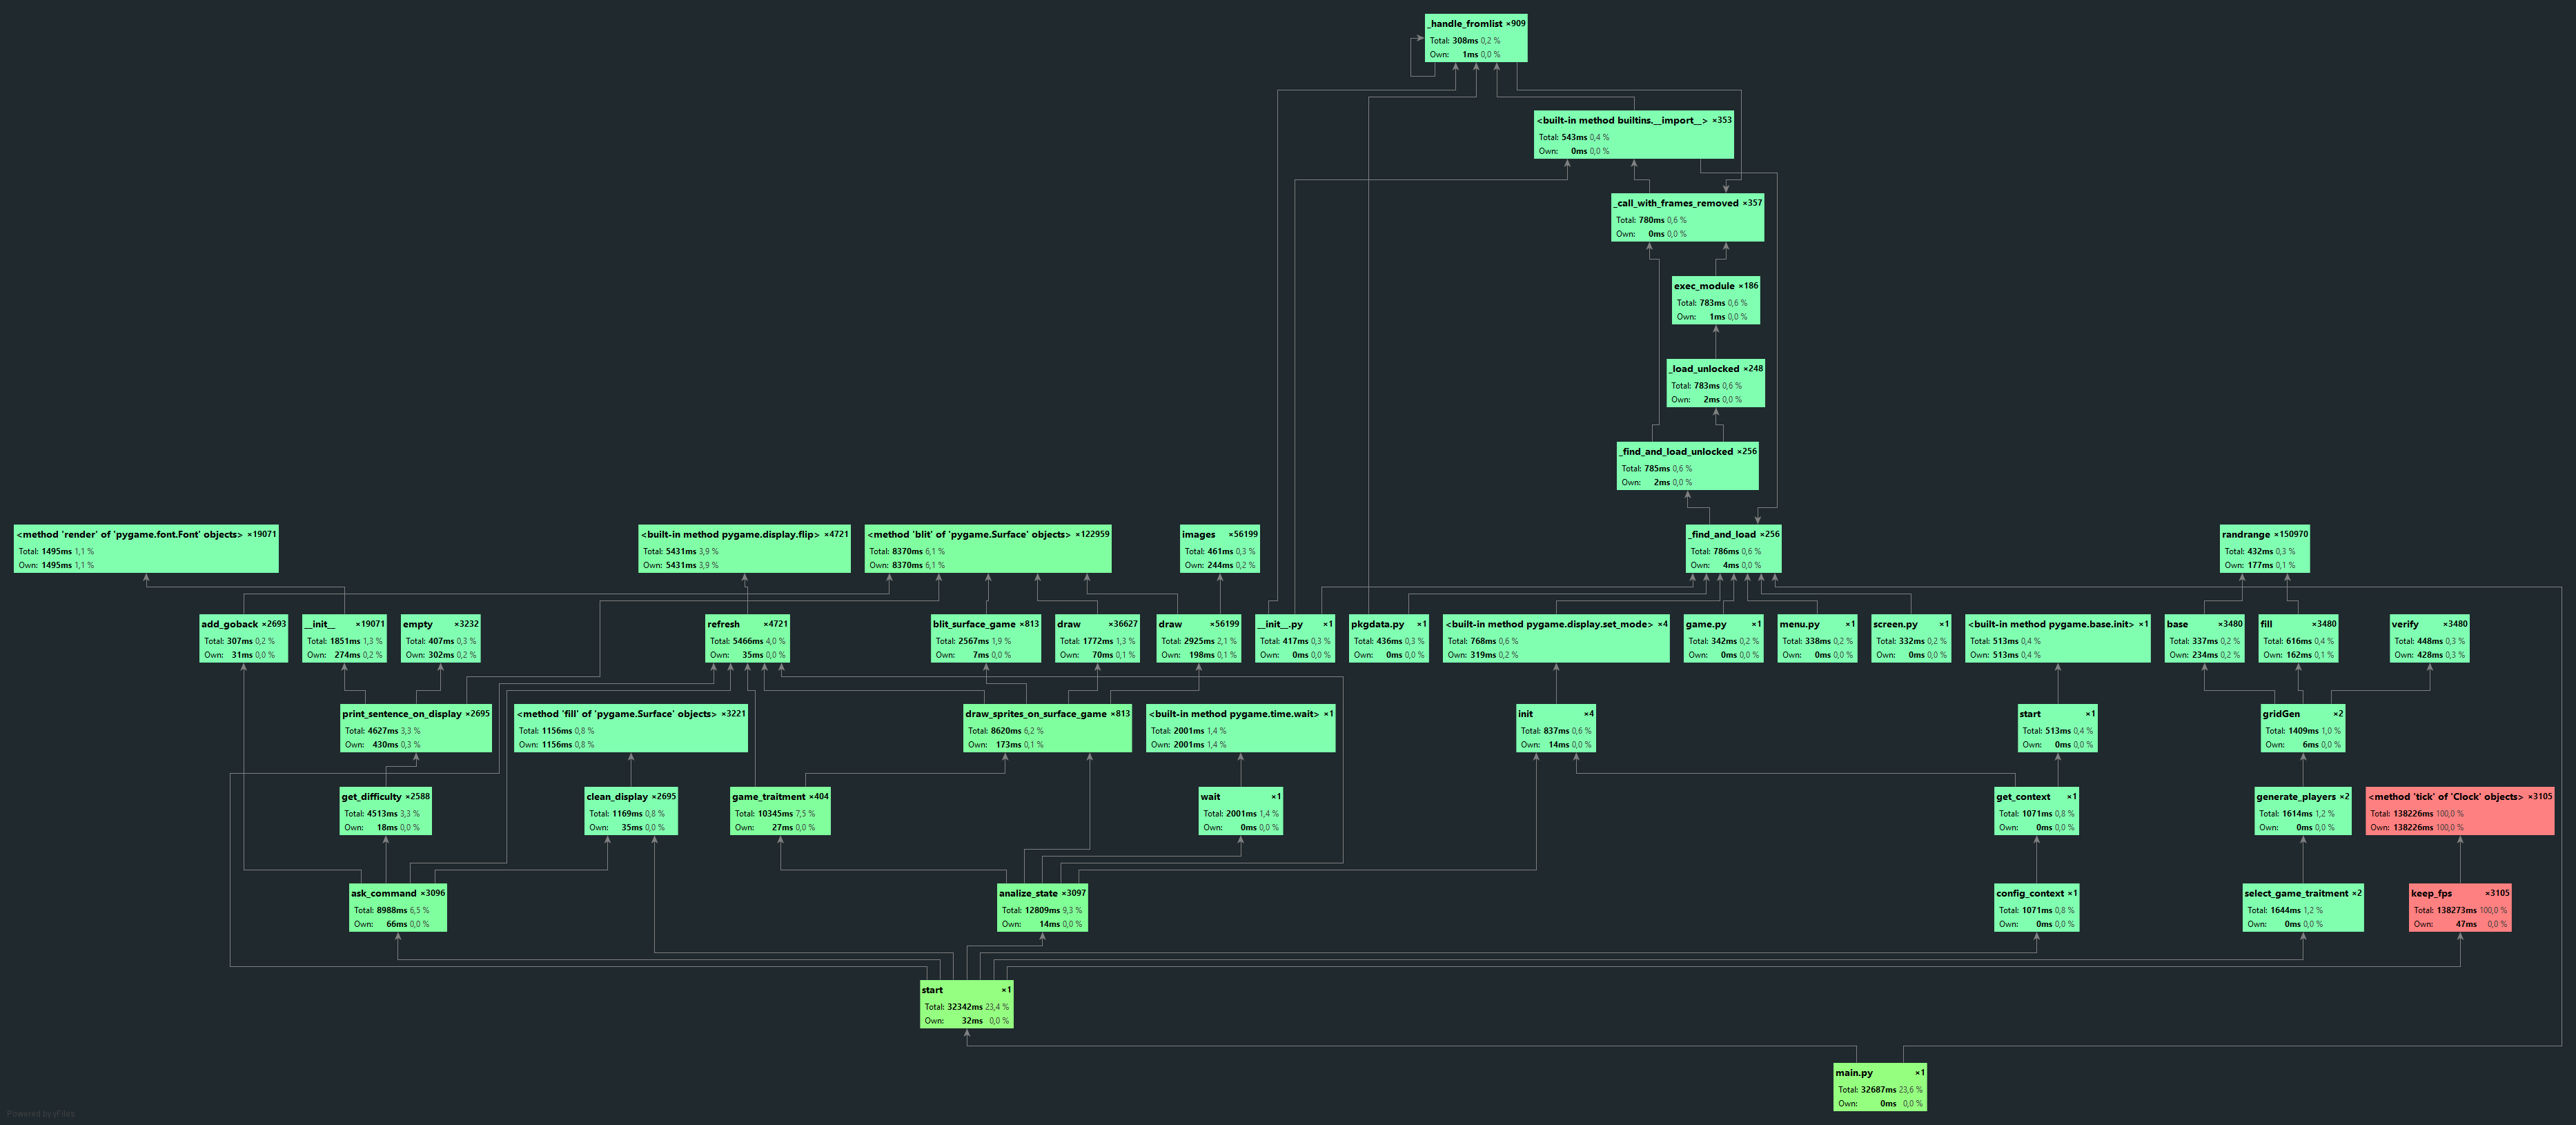
\includegraphics[width=\linewidth, height=2in]{Illustrations/graphJetBrains.png}
\caption{Graphique de structure de données}
\label{fig::graph}
\end{figure}

\subsection{Exécution}

\begin{figure}[H]
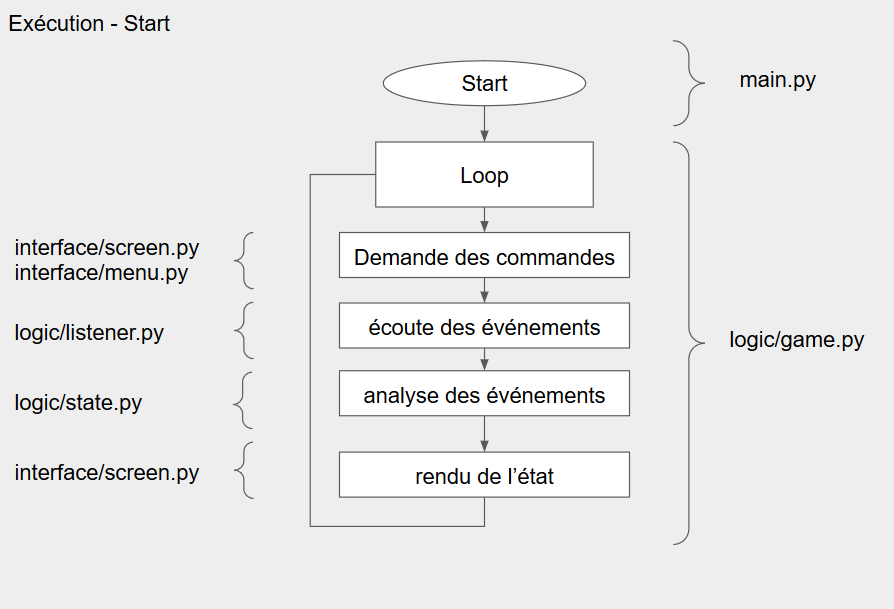
\includegraphics[width=\linewidth]{./Illustrations/execution.png}
\caption{Croquis de l'exécution du programme.}
\end{figure}

\subsection{Bibliothèques utilisées}

Voici la liste des bibliothèques externes utilisés :

\begin{itemize}
  \item{heapq}
    \begin{itemize}
      \item{Permet de créer une file prioritaire pour l'algorithme A*}
    \end{itemize}
  \item{Pygame}
    \begin{itemize}
      \item{Moteur graphique utilisé dans le projet.}
    \end{itemize}
\end{itemize}

\newpage

\section{Expérimentations}
\subsection{Mesures de performances}

Nous avons utilisé plusieurs outils pour mesurer les performances de notre programme, dans un premier temps, nous avons vérifié, quelles fonctions demandent le plus de temps de calcul grâce à un outil intégré à pyCharm.\\
Ce graphique (figure \ref{fig::graph}) nous permet de voir que la fonction keep\_fps (interface/screen.py) nous prend beaucoup de temps de calcul. Nous avions décidé de la supprimer mais cela faisait monter énormément l'utilisation processeur par notre programme(voir figure \ref{figure::forteconso}).

\begin{figure}[H]
 \centering
 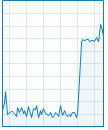
\includegraphics{Illustrations/gestionnaire_tache_forte_conso.png}
\caption{Utilisation du cœur après suppression de keep\_fps}
\label{figure::forteconso}
\end{figure}

Les mesures de performances ont été effectuées en obligeant le programme à utiliser un cœur précis (le numéro 7 par exemple) du processeur afin d'être le plus précis possible.\\

Cela demandait 60\% à 70\% des ressources d'un cœur ayant une vitesse de base de 3.6 Ghz.\\
Nous avons donc réintégré cette fonction à notre programme, et il est maintenant compliqué de constater une différence d'utilisation du processeur au moment où on lance le programme. En effet , le but de keep\_fps était de bloquer de nombre d'images par secondes à 20, il est donc normal que son temps d’exécution soit le plus long du programme. Au niveau de l'utilisation de la mémoire vive, le programme ne dépasse pas les 35 Mo.
Par conséquent, tout pc pouvant afficher un bureau est capable de lancer de manière fluide Sokoban.


\subsection{Difficultés rencontrés}

Le générateur de niveau et le solveur furent les parties les plus compliquées à réaliser.

Pour le générateur, il ne s'agit pas de placer des éléments de décor au hasard car il faut que chaque niveau soit réalisable que ce soit par le joueur que par le solveur ainsi que le personnage ou les caisses n'apparaissent pas dans un endroit ou ils seraient bloqués. Pour plus d'informations sur son fonctionnement, referez-vous à la partie dédiée: (\ref{gen}).

Concernant le solveur, il fallait trouver une solution complète sans changer la disposition du niveau, nous vous en parlons en détail dans la partie \ref{section::solveur}.

\newpage

\section{Conclusion}
\subsection{Récapitulatif}

Le jeu terminé, nous étions plutôt contents de nous. Nous avons en effet réussi à atteindre l'objectif fixé, mis à part quelques petits inconvénients (cf \ref{ameliorations}. Nous avons en effet réussi à produire un jeu totalement fonctionnel. Il est non seulement possible de jouer à deux mais aussi de jouer contre son propre ordinateur. Certaines fonctionnalités telles que le comptage des points ou bien la sélection possible de plusieurs niveaux a aussi permis d'ajouter beaucoup de contenu au jeu.Bien que lent pour la génération de certains niveaux aléatoires, le jeu tourne très bien. Un ordinateur peu puissant est en mesure de l'exécuter sans problèmes de performances. L'objectif principal a donc été largement atteint puisque le jeu est parfaitement fonctionnel et que différentes fonctionnalités supplémentaires on pu être ajoutées. Ce fut donc en somme un très bonne expérience qui nous a permis à tous de mettre nos connaissances en commun, et de progresser aussi bien individuellement que collectivement. 

\subsection{Améliorations possibles}
\label{Améliorations}

Nous allons répertorier ici les améliorations auxquelles nous avons pensé mais qui n'ont pas pu se réaliser, notamment par manque de moyens.
\begin{itemize}
\item Un solveur plus efficace.\\
Le solveur que nous avons conçu prend en charge un certain nombre de niveaux mais ne peut pas tous les résoudre. Nous avons fait en sorte que tous les niveaux du jeux soient résolvables pour pallier à ce problème. Malgré tout, il aurait été appréciable que le solveur puisse être en mesure de résoudre n'importe quel niveau qui lui soit présenté. De plus il est possible sur certains niveaux (comme le niveau 2) que le joueur réussisse à faire moins de déplacement que le solveur, il y a donc quelques améliorations possibles.
\item Un générateur plus rapide\\
Le générateur quand à lui peut générer n'importe quelle grille jouable en suivant certains paramètres. Le problème réside dans le temps qu'il lui faut pour arriver à créer une grille jouable. On pourrait éviter ce problème en générant une grille suivant des patterns (motif prédéfinis de grille). Ainsi une grille se générerait plus rapidement mais ne serait plus vraiment aléatoire puisque le fait d'ajouter des patterns sous-entend que ceux-ci on déjà été défini par avance. De plus, on pourrait se retrouver en présence de grilles lassantes puisqu'un même pattern pourrait apparaître plusieurs fois. Une connaissance plus poussée de Python aurait donc sûrement pu permettre d'optimiser le générateur.
\end{itemize}


\appendix

\end{document}
